\chapter{Introduction}
\label{ch:introduction}

\section{The Earth’s radiation budget}
The Earth's climate is driven by the energy flow into and out of the system. The incoming solar radiation (yellow fluxes in \figref{fig:earth_energy_budget}) reaches the Earth at the top of the atmosphere (TOA), then goes through the atmosphere and arrives at the Earth surface. During this process, approximately two thirds of this shortwave (SW) radiation is absorbed by the Earth surface and atmosphere, and roughly one third of this energy is reflected back to space. The the surface and atmosphere are heated by this incoming solar radiation, and they also re-emit the longwave (LW) radiation (purple fluxes in \figref{fig:earth_energy_budget}) to keep a relatively stable temperature. Globally, the annual mean incoming solar radiation flux at the TOA is about 340 W m$^{-2}$, the reflected solar radiation flux is around 100 W m$^{-2}$ and the outgoing longwave radiation (OLR) is close to 240 W m$^{-2}$ for period 2000--2010 \citep{Stephens2012update}. These three components balance with each other, but according to the observation, there is in fact a small positive imbalance (about 0.6 W m$^{-2}$) at the TOA.

\begin{figure}[ht]
	\centering
	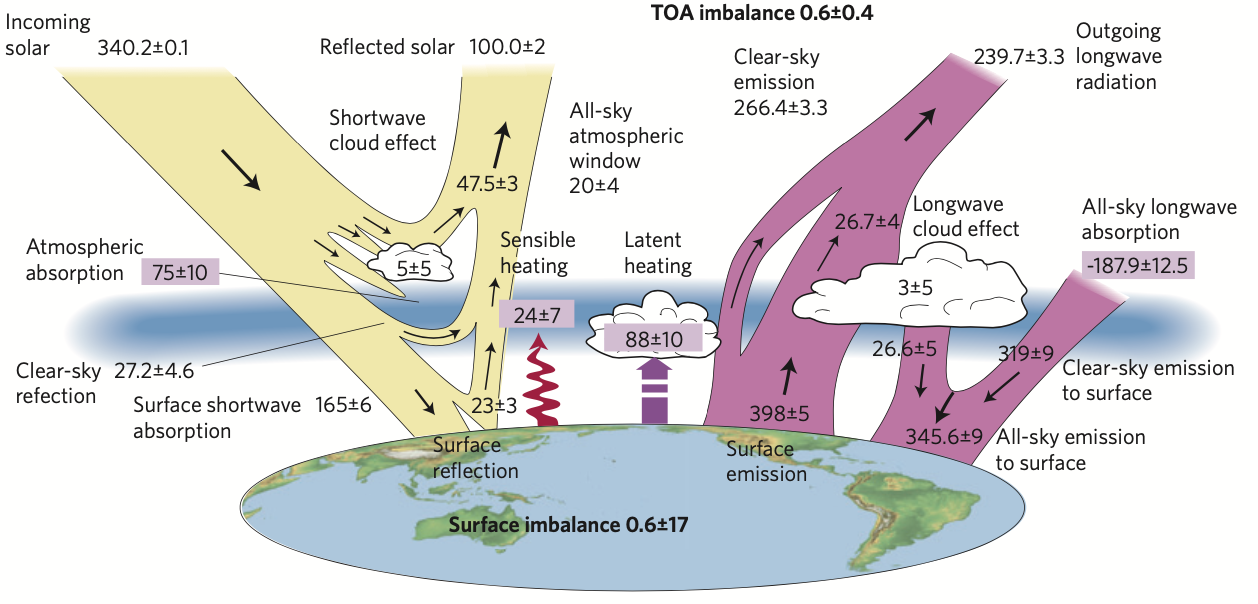
\includegraphics[width=1\linewidth]{{figs/literature_review/earth_enery_budget_Stephens2012}.png}
	\caption[The global annual mean energy budget of Earth for the approximate period 2000–2010 from \cite{Stephens2012update}]{The global annual mean energy budget of Earth for the approximate period 2000–2010. All fluxes are in Wm$^{-2}$. Solar fluxes are in yellow and infrared fluxes in purple. The four flux quantities in purple-shaded boxes represent the principal components of the atmospheric energy balance. Adapted from \cite{Stephens2012update}.}
	\label{fig:earth_energy_budget}
\end{figure}

\section{Cloud radiative effect}


\begin{figure}[ht]
	\centering
	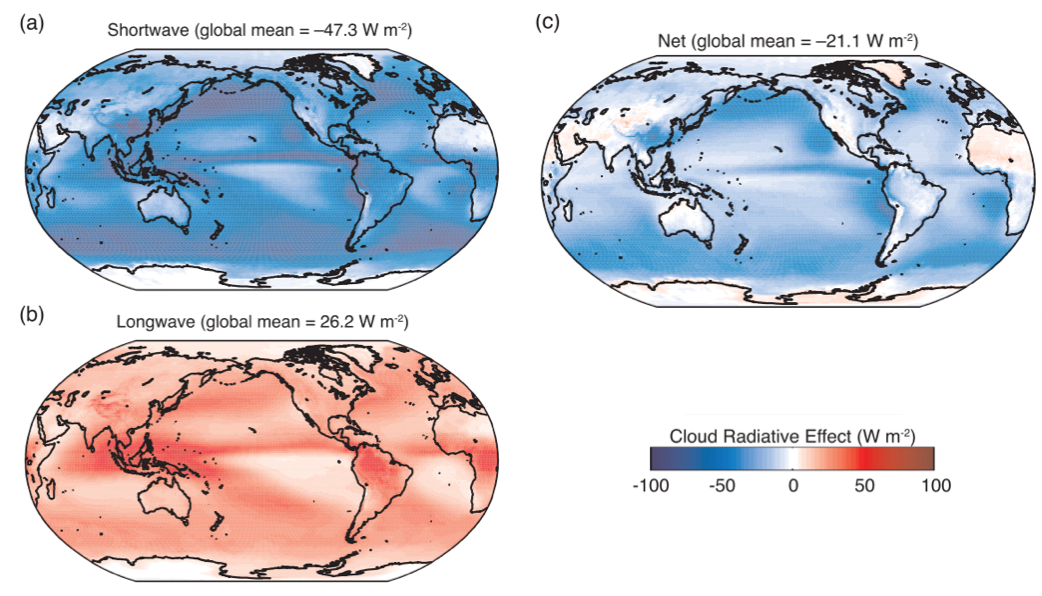
\includegraphics[width=1\linewidth]{{figs/literature_review/spatial_pattern_of_CRE_from_IPCC_ch7}.png}
	\caption{Distribution of annual-mean top of the atmosphere (a) shortwave, (b) longwave, (c) net cloud radiative effects averaged over the period 2001–2011 from the Clouds and the Earth’s Radiant Energy System (CERES) Energy Balanced and Filled (EBAF) Ed2.6r data set. Adapted from Fig. 7.7 of The Fifth Assessment Report (AR5) of the Intergovernmental Panel on Climate Change (IPCC) \citep{stocker2013climate}.}
	\label{fig:CRE_from_IPCC}
\end{figure}

\section{Cloud feedback}

\section{Cloud scheme}

\section{Research questions and thesis outline}
\label{sec:thesis_layout}
